% tae_submission.tex — rebuilt 2026-08-24 from the verified artifact set after
% the loss of the original source. Structure: SCAFFOLD_GO_BRIEF.md. Prose: the
% 51 recovered NOW blocks (Aug 20 patch set), with the Aug 24 memo v2 applied
% on top, in that order. Every number traces to a repo/Hub artifact; sweep and
% session labels are in the text by rule, not by exception.
%
% REQUIRES: neurips_2026.sty from the TAE workshop page (the REAL file, not a
% stub) placed alongside this file. The template's Times is kept; only the
% typewriter face is remapped (\ttdefault=lmtt), because the default tt emits Type 3
% bitmap fonts and arXiv flags the submission.
\documentclass{article}
\usepackage[dblblindworkshop]{neurips_2026}
\renewcommand{\ttdefault}{lmtt} % Type 1 typewriter; keeps the template's Times
\usepackage[T1]{fontenc}
\usepackage[utf8]{inputenc}
\usepackage{booktabs}
\usepackage{amsmath}
\usepackage{graphicx}
\usepackage{xcolor}
\usepackage{microtype}

\title{Reliable and Invalid: Entropy Collapse Separates a Verifiable Reward
  from the Construct It Proxies}
% NOTE: \workshoptitle is invisible in submission mode but PRINTS on the
% camera-ready ([dblblindworkshop, final]) --- set it per venue before any
% non-TAE build.
\workshoptitle{TAE (Trust-AI-Eval): Can We Trust AI Evaluation?}

\begin{document}
\maketitle

\begin{abstract}
Verifiable rewards are trusted because they are deterministic: a program
either awards the points or it does not. We post-train Qwen2.5-7B-Instruct
with GRPO on NYT Connections under a reward with a cheap structural component
(well-formed output) and an expensive semantic component (correct
groupings). On a strictly chronological test set of 162 puzzles (648 group
slots), capability moves in four stages: the untrained Instruct model
recovers 26 group slots, supervised fine-tuning 56, the step-50 GRPO
policy 77, and the step-403 endpoint 4 (the middle arms re-serve at 52 and
80 in later sessions; the endpoints reproduce exactly) --- against a
1.4-slot chance floor for a uniformly drawn valid partition. Step 50 improves on the untrained model by a
paired $+0.315$ $[+0.204, +0.438]$ on the 0--4 scale; step 403 falls below it
by $-0.136$ $[-0.191, -0.080]$, a deficit that reproduces across three
seeds (all three point estimates inside that interval). The
\emph{training} reward reads the collapse as success: it climbs 0.99 to
its 1.6 ceiling between steps 100 and 125 --- inside the
collapse window --- and across-rollout variance hits zero there on nearly
every prompt; both in-sample signals bracket the turn, neither signs it.
The identical reward evaluated out of sample records the
reversal: 0.246 at step 50, 0.266 at step 100 (separate serving session),
0.125 at the end, against the untrained model's 0.165. The semantic peak
arrives by 5.7\% of the run's
eventual KL displacement; the remainder undoes it as policy entropy collapses
and structural validity rises. The collapse survives disabling TRL's
group-level reward normalization, and three LLM judges scoring the test
generations blind all rank step 50 above the untrained model above the final
policy --- placing the \emph{most} well-formed arm last. At 1.5B no arm is
distinguishable from that chance floor, so the scale contrast reports what the
reward did to the verifiable component and makes no claim about the
construct. We read this
as a construct-validity failure: the in-sample metric cannot locate the
point at which a verifiable reward stops helping; the same reward, held
out, brackets it.
\end{abstract}

\section{Introduction}
\label{sec:intro}

Post-training against verifiable rewards is attractive for a reason that
sounds decisive: the reward is a program. It returns exactly what it was
written to return, and the argument that this
buys immunity from reward hacking\footnote{We follow the common usage
\emph{reward hacking} throughout; \citet{skalse2022}, whose formalization we
adopt, publish it under the name \emph{reward gaming}.} rests on that
reliability. This paper is about the gap reliability does not close: the gap
between the reward and the construct it stands in for. We train on NYT
Connections --- sixteen words, partitioned into four groups of four ---
chosen because well-formedness and correctness are unusually separable: a
response can be a perfectly valid partition of the board and completely
wrong. Our reward pays for both, asymmetrically; two of its five components
can be checked by reading the string, three require the answer key.

For fifty steps it works. Held-out groups recovered run $26 \rightarrow 56
\rightarrow 77$ across the untrained Instruct model, the supervised checkpoint
GRPO is initialized from, and step 50 --- a split of $+26$ to $+30$
supervised against $+21$ to $+28$ reinforcement learning across serving
sessions, overlapping ranges the data do not resolve
(\S\ref{sec:arc}). Over the following
353 steps the same run falls to 4 slots, below the untrained model and near
the 1.4-slot floor of a uniformly drawn valid partition, while
the invalid-output rate falls by an order of magnitude and the training
reward reaches its 1.6 maximum and averages 1.5814 thereafter, with
zero variance across the $K=8$ rollouts on $\sim$95\% of prompts. A
practitioner watching that curve saw a solved task. The same reward
function, evaluated on data the policy was not updated against, ranks all
three checkpoints correctly. The failure is not in the metric; it is in the
universal practice of reading it in sample.

\paragraph{Contributions.} A fully verifiable, temporally
leakage-controlled case study in which GRPO first improves and then destroys
the target construct, ending below the untrained Instruct model across three
seeds (\S\ref{sec:arc}); a checkpoint-level account placing the semantic
peak at or before 5.7\% of the run's KL displacement, co-occurring with
entropy collapse and with the training reward at its ceiling --- zero group-relative
advantage on $\sim$95\% of prompts --- from step 125 onward
(\S\ref{sec:mechanism}); an ablation showing the collapse survives
disabling TRL's group-level reward normalization
(\S\ref{sec:ablation}); a blind LLM-judge evaluation showing the reversal
is legible from outside the reward (\S\ref{sec:judge}).

\section{Task, pipeline, and the reward's asymmetry}
\label{sec:setup}

\paragraph{Task and data.} 1{,}078 dated NYT Connections puzzles (1{,}077
after validation), split strictly chronologically: 807 train (2023-06-12 to
2025-08-27), 108 validation, 162 test (2025-12-15 to 2026-05-29). Every test
puzzle postdates every training puzzle; regressing groups-correct on puzzle
date across the test window yields slopes indistinguishable from zero for
both the untrained Instruct model ($-0.158$ groups/year $[-0.634, +0.292]$) and the trained
policy ($+0.035$ $[-0.271, +0.329]$), so the split controls contamination;
we cannot detect drift, though the intervals are wide (a 5.5-month window,
slopes per year) and only large drift would show.

\paragraph{Pipeline.} Qwen2.5-7B-Instruct (and 1.5B for the scale contrast),
rank-16 LoRA. SFT for 3 epochs on the training split, then GRPO
\citep{deepseekmath} from the SFT checkpoint: $K=8$ sampled completions per
puzzle at temperature 0.9, group-relative advantages, $\beta=0.001$ against
the SFT reference, learning rate $5\times10^{-6}$, one epoch (403 optimizer
steps) at 7B.

\paragraph{The reward.} Table~\ref{tab:reward} is the crux of the paper.

\begin{table}[h]
\centering
\caption{The reward decomposition. Two components are verifiable from the
emitted string alone; three require the answer key. The policy is trained on
the sum.}
\label{tab:reward}
\begin{tabular}{lcl}
\toprule
Component & Value & Cost to check \\
\midrule
Parses as four groups of four & $+0.1$ & \textbf{cheap} --- read the string \\
Correct groups & $+1.0 \times (\text{correct}/4)$ & needs the answer key \\
All four groups correct & $+0.5$ & needs the answer key \\
Group with exactly 3 correct words & $+0.05$ & needs the answer key \\
Invalid output & $-0.1$ & \textbf{cheap} --- read the string \\
\bottomrule
\end{tabular}
\end{table}

Maximum 1.6. The model can raise its score two ways: by getting better at
the puzzle, or by getting better at emitting well-formed output. Only one of
those is the construct. That asymmetry --- cheap and expensive components,
independently satisfiable --- is the design property this paper studies.

\section{The arc on held-out data}
\label{sec:arc}

Table~\ref{tab:arc} reports the three checkpoints of the reported 7B run on
the 162-puzzle test set, greedy decoding, all three arms served in a single
vLLM session so every comparison is within-session.

\begin{table}[h]
\centering
\caption{7B on the test split (162 puzzles, 648 group slots; one serving
session; greedy). Means on the 0--4 scale are exact ratios of the count
column. Bootstrap intervals are percentile, seed 0.}
\label{tab:arc}
\small
\setlength{\tabcolsep}{4pt}
\begin{tabular}{lccccc}
\toprule
Arm & Groups correct (0--4) & Groups (of 648) & Invalid & Mean reward & Solves \\
\midrule
Instruct (untrained) & 0.1605 $[0.105, 0.222]$ & 26 & 6.8\%  & 0.165 & 0/162 \\
\textbf{GRPO, step 50}  & \textbf{0.4753} $[0.364, 0.599]$ & \textbf{77} & \textbf{16.7\%} & \textbf{0.246} & 2/162 \\
GRPO, step 403     & 0.0247 $[0.000, 0.056]$ & 4 & 0.6\%  & 0.125 & 0/162 \\
\bottomrule
\end{tabular}
\end{table}

Two reference points frame the table. A uniformly drawn valid partition
recovers $4 \times 5775/2{,}627{,}625 = 0.0088$ groups per puzzle, or
\textbf{1.4 slots} across this split; the step-403 endpoint sits at 2.8
times that floor --- near enough that
``below the untrained model'' and ``near a random valid partitioner'' describe
the same policy. Second, GRPO was initialized from the supervised checkpoint,
not the untrained model. That checkpoint decodes to \textbf{56 slots} (0.346)
in one serving session and 52 (0.321) in another (2 of 162 puzzles;
Appendix~\ref{app:endpoints}), and step 50 itself decodes to 77 or 80 by
session (below), so the stage accounting is $26 \rightarrow 52\text{--}56
\rightarrow 77\text{--}80 \rightarrow 4$. The two middle arms never shared
a serving session, so every stage split crosses sessions: over the four
pairings, SFT contributes $+26$ to $+30$ and GRPO $+21$ to $+28$ ---
overlapping ranges, and the data do not resolve which stage contributes
more.

The method works, then reverses: $+0.315$ $[+0.204, +0.438]$ paired against
the untrained model at step 50, $-0.136$ $[-0.191, -0.080]$ at step 403, both
intervals excluding zero.
Means in Table~\ref{tab:arc} are exact ratios of the count column; we
report both. Two details locate the
mechanism. Held-out mean reward reads 0.246 at step 50 and 0.125 at step
403, against base's 0.165, all in one session; in the later session of the
plateau paragraph below, step 100 reads 0.2664 to a step-50 re-serve's
0.2525 --- the highest held-out reward the reported run produced: the
reward peak, like the groups peak, is a plateau. The training reward meanwhile reaches its ceiling by
step 125 (\S\ref{sec:mechanism}): the same reward ranks the checkpoints
correctly out of sample and fails to on the training curve, and that
contrast --- not the reward's determinism --- is this paper's subject. And
the step-50 policy is worse than base on structure (16.7\% invalid against
6.8\%) but \emph{not} worse than its actual initialization, the SFT arm at
22.2\% --- so what is specific to the phase after step 50 is the semantic
collapse, not the structural climb, which was already more than half
complete before the peak (\S\ref{sec:mechanism}).

\paragraph{The peak is a plateau, not a knife edge.} Step 100 of the same
run was additionally evaluated on test, in a single later serving session
alongside a re-serve of step 50: 76/648 groups recovered (0.4691) against
step 50's 80/648 (0.4938)
\emph{in that session}, paired difference $-0.0247$ $[-0.1481, +0.0927]$
($n=162$, seed-0 bootstrap) --- statistically indistinguishable. The peak spans at least
steps 50--100; the collapse occurs between steps 100 and 150, where the
validation semantic score falls from 35/400 to 3/400 on the $n=100$
temperature-0.9 entropy sweep (\S\ref{sec:mechanism}).

\paragraph{Reproducibility across serving sessions.} Base and the final
checkpoint reproduce per-puzzle \emph{exactly} across three independent
vLLM sessions (0 of 162 differences each). The step-50 checkpoint does not:
it differed on 2/162 puzzles across sessions (77 vs.\ 80 of 648) and on
6/162 completions between two greedy passes within one session.
Mid-training policies sit near argmax ties that batched inference resolves
inconsistently; converged ones show none. That is evidence \emph{for}
the entropy account, and it is why every step-50 number in this paper
carries its serving session. The published headline (77/648) is the
original single-session evaluation; the plateau comparison above uses the
later session's within-session pair.

\paragraph{Robustness of the endpoint.} Three independent 7B seeds land at
4, 7 and 11 recovered slots of 648 ($0.045 \pm 0.022$ on the 0--4 scale) ---
all below base's 26. Their LoRA update directions agree pairwise: cosine
$+0.67$ to $+0.69$ between merged weight-delta directions --- read
descriptively, as three runs finding the same attractor; seeds sharing an
initialization and dataset are not isotropic draws, so no random-direction
null applies. Best-of-16 sampling does
not rescue the converged policy, which is what a collapsed-entropy account
predicts --- a near-deterministic model has nothing new to sample; the
single-seed pass@16 contrasts, read as illustrative only, are given with
the per-arm values in Appendix~\ref{app:endpoints}.

\paragraph{Conditioning on well-formed output widens the gap rather than
explaining it, and we label the operation for what it is.} A reviewer will
ask whether the effect is an artifact of validity, since invalid generations
score zero groups, and validity is what GRPO improved. Restricting to
structurally valid generations at 7B, each arm's conditional computed within
a single serving session (the SFT arm's is its 56-slot session): base
\textbf{0.172} ($n=151$ of 162),
SFT \textbf{0.444} ($n=126$), GRPO \textbf{0.025} ($n=161$). This is a
rescaling and we label it as one: each conditional value is that arm's
unconditional mean divided by its validity rate, exactly, so the gap widens
automatically whenever the low-scoring arm is the more valid one, which here
it is by construction. What the rescaling licenses is only the negative
claim, the one we need: the deficit survives with formatting held fixed.
Among answers that parse, the converged policy recovers 4 group slots where
the untrained model recovers 26. (The 1.5B conditionals, on underlying
counts of 1, 2 and 1, are given in Appendix~\ref{app:small}.)

\paragraph{One prediction of our own account fails, and we report it.} If
entropy collapse selectively destroyed board-specific inference, the loss
should concentrate in the strata that need the most inference. It does not:
across the 158 of the 162 test
puzzles that carry a single stratum label, relative loss from the untrained
model to GRPO runs 92\% on \texttt{category} ($n=69$), 67\% on
\texttt{cultural} ($n=28$), 86\% on \texttt{tag-fillin} ($n=40$) and 100\% on
\texttt{wordplay} ($n=21$, from a near-floor base of 0.048, i.e.\ a single
recovered slot). That is closer to uniform destruction than to a gradient.
We report it as a failed prediction of the selective-inference
story rather than a refutation: at these stratum sizes the spread cannot
separate uniform loss from a graded one.

\section{The scale contrast at 1.5B}
\label{sec:scale}

At 1.5B the instrument reads nothing. The untrained model recovers one group
slot of 648, GRPO recovers one, and SFT --- the best arm --- recovers two,
against the chance floor of 1.4 slots established in
Section~\ref{sec:arc}. No arm is distinguishable from that floor --- SFT's
two slots carry an exact binomial interval of $[0.0015, 0.0444]$ on the 0--4
scale (Appendix~\ref{app:small}), which
contains it --- so no claim about whether the construct was preserved is
available at this scale. What is visible is that the reward did
at 1.5B what it did at 7B on the component it can verify, driving invalid
output from 32.1\% to 2.5\% and mean reward from 0.049 to 0.113 (full table
in Appendix~\ref{app:small}). We report this as an observation rather than a
contribution. The runs are epoch-asymmetric --- 806 optimizer steps, two
epochs, at 1.5B against 403 steps and one epoch at 7B --- and we have no 1.5B
checkpoint trajectory, so ``the construct was untouched at 1.5B'' would be a
claim about an endpoint, which is exactly what this paper shows cannot settle
such a question.

\section{Mechanism: entropy collapse and the step-50 semantic peak}
\label{sec:mechanism}

Figure~\ref{fig:mechanism} scores checkpoints of the reported run on the
$n=100$ temperature-0.9 \emph{entropy sweep} (denominators of 400; full
per-checkpoint values in Appendix~\ref{app:ckpt}). The ablation's
\emph{checkpoint sweep} in \S\ref{sec:ablation} is $n=108$, greedy,
denominators of 432; the two are different measurements and are never
mixed.

\begin{figure}[t]
\centering
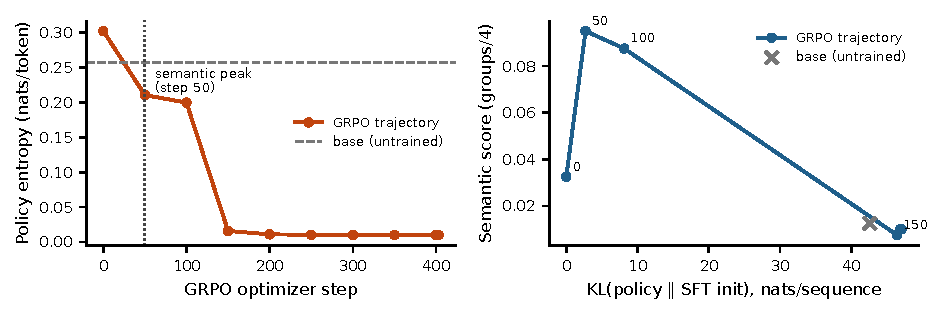
\includegraphics[width=\linewidth]{../figs/fig1_entropy_collapse.pdf}
\caption{The mechanism, on the $n=100$ temperature-0.9 entropy sweep
(reported 7B run, seed 0). \textbf{Left:} policy entropy against optimizer
step --- a 30-fold collapse, with the cliff between steps 100 and 150.
\textbf{Right:} semantic score against KL from the SFT initialization, the
over-optimization curve: the peak arrives by 2.70 of an eventual 47.05 nats
per sequence (5.7\% of the run's displacement; step 50 is the earliest
checkpoint retained), and the remaining 94.3\%
undoes it. The untrained Instruct model is plotted as an off-trajectory
reference at 42.60 nats: KL from the initialization measures displacement,
not damage (\S\ref{sec:mechanism}).}
\label{fig:mechanism}
\end{figure}

The semantic peak has a location; the structural climb does not. The
semantic score rises from 0.0325 at the SFT initialization to 0.0950 at step
50 (13/400 to 38/400 recovered slots), then falls to 0.0075 by step 150
and holds at 0.0100 from step 200 on, never re-approaching the peak. The
structural score (fraction of valid partitions, not
shown in Fig.~\ref{fig:mechanism}) climbs
across the same window and past it, with one reversal: 0.37 at the SFT
initialization, 0.68 at step 50, 0.64 at 100, 0.95--0.96 from 150 on; of
the 0.59 total structural gain, 0.31 is banked by step 50, concurrent with
the semantic peak.

The trajectory is therefore not a trade with a turning point: it is a broadly
monotone structural climb --- one reversal, at step 100 --- with a semantic
hump on top, and only the hump has a location. One instrumentation gap
qualifies the shape: no checkpoint exists between steps 100 and 150 ---
81\% of the eventual KL displacement (8.12 to 46.42 nats) falls in that
window --- so the descent's steepness and the turn's location are
interpolated, not measured. The entropy account survives this reading unchanged ---
it predicts a policy that ends reliably well-formed and adaptively wrong,
which is what the endpoint is --- but it does not license the vocabulary of
a trade and we do not use it.

\paragraph{Entropy collapse co-occurs with the loss.} Policy entropy falls 13.4-fold
between steps 50 and 150, the window in which the semantic score falls
12.7-fold; by step 150 the policy is effectively deterministic. A
near-deterministic policy can be reliably well-formed --- the format is the
same for every board and can be satisfied without reading the puzzle.
Per-prompt determinism does not preclude board-specific
correctness --- within-prompt entropy and across-prompt conditioning are
independent, and on the training prompts visited after step 125 this policy
earns mean reward 1.5814 with identical rollouts on $\sim$95\% of them.
What the collapse removes is within-prompt variation: nothing new to sample
(the pass@16 result), no group-relative learning signal (the zero-advantage
fraction). What survives on held-out boards is the reward's
input-independent component --- measured, not asserted: the cheap
structural term, $0.1(1-2\cdot\text{invalid rate})$ from
Table~\ref{tab:arc}, is 52\% of the untrained model's held-out reward,
27\% of step 50's, and 79\% of the endpoint's --- the decomposition
\S\ref{sec:implications} recommends, applied to our own data. Whether what
survives on \emph{training}
boards is the memorized key is \S\ref{sec:limitations}'s open question.
An argument for plausibility, not
a demonstrated mechanism: along this single path entropy, KL, structural
validity and the zero-advantage fraction move together, and we never
intervened on entropy (\S\ref{sec:limitations}).

\paragraph{KL is the budget view, and it is a path length, not a damage
scale.} The step-50 checkpoint sits 2.70 nats
from the SFT initialization and is, jointly with step 100
(\S\ref{sec:arc}), the best policy this run produced on
held-out data. The run spent 47.05: 77 slots at 5.7\% of
the displacement, 4 at all of it.
Two qualifications keep this a path description, not a scale.
Step 50 is the earliest non-initial checkpoint retained (nothing was
measured at steps 10--40), so ``at 5.7\%'' means \emph{at or before} it.
And KL from the initialization measures displacement, not damage: the
untrained Instruct model sits 42.60 nats out on the same estimator ---
90.5\% of the run's displacement --- while scoring 0.0125 on this sweep
(Appendix~\ref{app:ckpt}). Each estimate is taken under its own policy's
samples, so base is far from SFT along a different direction, not a point
on this trajectory; 5.7\% dates the peak within this run and licenses no
reading of KL as distance toward degeneracy. The sweep also compresses
base's margin over the endpoint (5/400 vs.\ 4/400, where the greedy test
instrument reads 26 vs.\ 4): temperature-0.9 sampling costs a high-entropy
policy far more than a collapsed one --- the instrument gap is the entropy
account in miniature.

\begin{figure}[t]
\centering
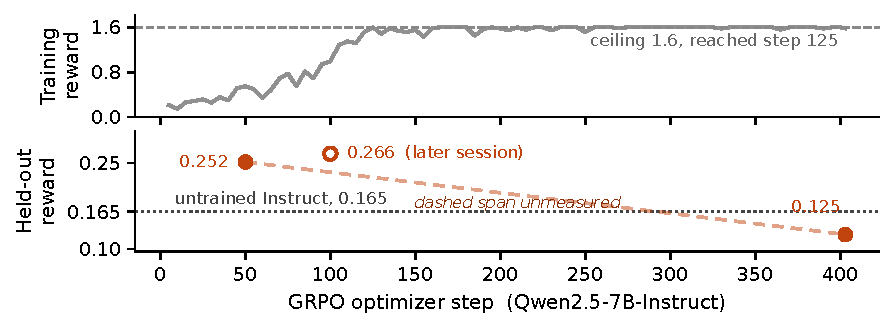
\includegraphics[width=\linewidth]{../figs/fig3_reward_curves.pdf}
\caption{The same reward function, in sample and held out (reported 7B run,
seed 0). The training reward (gray; sampled, $T{=}0.9$, $K{=}8$; TRL's
5-step interval averages)
first touches the reward function's ceiling of 1.6 at step 125 and averages
1.5814 from then on.
The held-out mean reward on the 162-puzzle test set (solid markers; greedy;
single
serving session) peaks at step 50 within its session and ends below the
untrained Instruct model.
The step-100 point (hollow marker) is from a later serving session --- 0.2664
there, against a step-50 re-serve at 0.2525 --- and is not joined to the
curve.}
\label{fig:rewards}
\end{figure}

\paragraph{The training signal, read from the trainer's own logs.} Figure
\ref{fig:rewards} shows the paper's central contrast on one axis: the
training reward first touches the reward function's ceiling of 1.6000 at step
125 and averages 1.5814 over the logged points from then on, with
excursions that shrink as training proceeds: the deepest is 1.4300 at step
155, and the residual gap to the ceiling closes at $+1.9\times10^{-4}$ per
step ($t=3.49$, $p\approx0.001$; Mann--Kendall agrees) --- the policy
keeps consolidating onto the ceiling
long after the group-relative signal is gone. What the figure cannot show is TRL's own
\texttt{frac\_reward\_zero\_std} diagnostic: the fraction of prompt groups
whose eight sampled rewards are identical, i.e., whose group-relative
advantage is exactly zero. It rises from 0.0 at step 50 to 1.0 at step 125
and averages 0.946 over the remainder of training, so from step 125 onward
the optimizer receives no learning signal on nearly every prompt. Read as
diagnostics, both in-sample signals bracket the collapse: the mean's
climb to ceiling (0.9931 to 1.6000, 41.8\% of its observed range) and the
variance's fall to zero both land between logged steps 100 and 125. Neither
supplies a sign --- saturation with zero spread is what mastery and
degeneracy alike look like --- so held-out evaluation still decides which.
Part of that climb is the instrument: training reward is measured under
temperature-0.9 sampling, and as entropy collapses sampled decoding
converges on greedy --- some of the rise is the sampling penalty vanishing,
not the policy changing (the sweep-vs-test gap above, read in the other
direction). That consolidation partly answers what drives the remaining
278 steps of movement while $\sim$95\% of prompts carry zero advantage:
the residual prompts still carrying signal keep pushing the policy onto
the ceiling; the weight-space counterpart of that push we have not
measured.

\paragraph{$\beta$ was numerically inert, and the bracket is not an
experiment.} An earlier configuration at learning rate $10^{-6}$ and
$\beta=0.04$ froze the policy (KL $\approx 0.001$ for 403 steps; greedy
outputs byte-identical to SFT). The reported configuration, at
$5\times10^{-6}$ and $\beta=0.001$, overshoots by roughly as much as the
first undershoots. We state two qualifications immediately, because both
weaken the pair as an experiment and neither weakens the observation.
First, the two configurations differ in \emph{two} variables at once,
$\beta$ by $40\times$ and the learning rate by $5\times$; a policy frozen
at the lower learning rate is the expected consequence of the learning rate
alone, so the pair bounds a region jointly and attributes nothing to either
variable individually, and we do not claim to have measured inside a KL
window. Second, $\beta=0.001$ was numerically inert throughout the
reported run: at step 50, $\beta \cdot \mathrm{KL} = 0.001 \times 2.70 =
0.0027$ reward units --- eighteen times smaller than the one-away
partial-credit term and 0.17\% of the 1.6 maximum --- and at convergence it
reaches 0.047. The KL reference never meaningfully restrained the policy
in the reported run, so this paper contains no evidence about what a KL
penalty does when it is large enough to matter, and the
intermediate-$\beta$ sweep remains unrun.

\section{The ablation: the collapse is not the normalization default}
\label{sec:ablation}

We inherited \texttt{scale\_rewards="group"} from TRL --- verified as the
default in trl 1.10.0, whose \texttt{GRPOConfig.\_\_post\_init\_\_}
normalizes \texttt{False} to \texttt{"none"}. Reviewers of an earlier
draft independently named it as a confound:
once the policy is near-deterministic, the within-group standard deviation
that the advantage is divided by approaches zero, amplifying sampling noise
into large updates --- which alone might produce the collapse, its timing,
and the cross-seed agreement. \citet{drgrpo} argue against this
normalization on independent grounds.

We reran the 7B pipeline identically --- same SFT warm start, learning
rate, $\beta$, $K$, temperature, LoRA rank, epoch count, seed --- with
reward scaling disabled, the resolved value read back off the constructed
trainer configuration. The signature is unchanged on the greedy
$n=108$ checkpoint sweep: validation semantic score rises to 62/432 at step
50, falls to 35/432 by step 100 and 4/432 by step 150, while structural
validity climbs 0.70 to 0.96. The validation-selected peak (step 50, frozen
before any test puzzle was scored) recovers 87/648 on test (0.5370
$[0.4134, 0.6668]$), $+0.377$ $[+0.247, +0.506]$ paired
against base. The final policy recovers 7/648 (0.0432 $[0.0123, 0.0804]$)
--- below base by $-0.117$ $[-0.179, -0.056]$ paired, and within $+0.019$
$[0.000, +0.043]$ of the original run's final policy.

The signature survives in the dynamics too, though not point for point:
without reward scaling, policy entropy falls 0.2111 (step 50) $\to$ 0.1346
(100) $\to$ 0.0128 (150) and stays near 0.011 through step 403 (original
endpoint 0.0099), while KL rises 2.75 $\to$ 17.84 $\to$ 45.64 nats per
sequence and plateaus near 46 (original: 47.05) --- twice the original's
8.12 at step 100, so intermediate magnitudes differ. On the $n=100$
temperature-0.9 entropy sweep --- a different measurement from the greedy
$n=108$ checkpoint sweep above --- semantic score reads 35/400 at step 50,
17/400 at 100, then 2/400 from step 150 onward. The hump, the collapse,
the entropy endpoint, and the below-base endpoint all survive with the
normalization off. The phenomenon is not a library default.

\section{The reversal is legible from outside the reward}
\label{sec:judge}

The 162 test generations from base, step 50 and the final policy were
scored blind --- board words and completion only, no answer key --- by
three LLM judges (gpt-5-mini, gemini-2.5-flash, claude-sonnet-4-5) on a
1--10 scale, 1458/1458 responses parsed. All
three rank step 50 above base above the final policy, and all nine pairwise
per-puzzle differences exclude zero under a paired bootstrap (seed 0);
step-50 minus final is $+0.60$ $[+0.44, +0.78]$, $+3.25$ $[+2.81, +3.67]$
and $+1.62$ $[+1.33, +1.90]$ respectively. That ordering rules out the
obvious confound: the final policy is the
\emph{most} well-formed arm on this split (0.6\% invalid against 6.8\% and
16.7\%), so a shared preference for well-formed text would have placed it
first, not last. Whatever the judges read, it is not the component the reward
can still distinguish. Judges do err in
correlated ways \citep{kohli2026}, so we read this as three correlated
readings of one external signal rather than three independent
confirmations; per-item Pearson $r$ across the three judge pairs is 0.456,
0.587 and 0.626 over all 486 items, lowest on the final policy's arm
(0.200 to 0.433). The nine comparisons form one family and we apply no
multiplicity correction; all nine intervals exclude zero by margins no
standard correction would close.

\section{Implications for evaluation practice}
\label{sec:implications}

\paragraph{Distinguish in-sample from held-out proxy metrics before
concluding a proxy has failed.} Evaluated on held-out data, our reward
ranks the three checkpoints correctly; it fails only in the form
practitioners actually consult it --- as a training curve, in sample, where
it reads perfect. One function, two measurements: in sample it is reliable
and invalid --- this paper's title; held out it carries what validity it
has. The cheap remedy is not a better reward. It is the
same reward, run on data the policy was not updated against --- plus the
trainer's own in-sample brackets, mean saturation and zero variance alike,
though neither signs the turn (\S\ref{sec:mechanism}).

\paragraph{Report reward components separately, never the aggregate.} The
failure is invisible in the sum and obvious in the decomposition, which
costs nothing: \S\ref{sec:mechanism} reports it for our three arms (52\%,
27\%, 79\%). Component decomposition is a standard
reward-model diagnostic; it is simply not applied to rewards that are
deterministic, because determinism is taken to have settled the question.

\paragraph{Treat single-seed RL results as uninterpretable.} Our own three
seeds span 0.025 to 0.068 at the endpoint. This applies with equal force to results
that come out well, including this paper's step-50 result: one seed,
selected as the argmax of a nine-point validation grid (step 100 scores
0.0875 to step 50's 0.0950 at $n=100$, inside one standard
error). The grid preceded every test evaluation of the selected checkpoint
(the ablation's peak was likewise frozen first), so this is ordinary
validation-based selection, and the step-100 evaluation
(\S\ref{sec:arc}) shows a plateau, not a lucky column.

\section{Related work}
\label{sec:related}

\paragraph{Reward-model overoptimization.} \citet{gao2023scaling}
established this curve shape --- gold-standard performance rising and then
declining as KL from the initialization grows --- for \emph{learned} reward
models, where the accepted explanation is Goodhart against an
approximation, remediable in principle with a better reward model
\citep{stiennon2020}. Our reward is a program: it
approximates nothing, and there is nothing in it to game. The curve
therefore requires only independently satisfiable cheap and expensive
components --- a design property, not a fit property --- and determinism is
the very feature cited to argue verifiable rewards escape this failure
mode.

\paragraph{RL for reasoning and entropy collapse.} Verifiable-reward RL
underlies recent reasoning systems \citep{deepseekr1, deepseekmath}.
\citet{yue2025} question whether RLVR extends capability beyond the
pre-trained base model's pass@$k$ ceiling; our reference point differs (an
instruction-tuned checkpoint, RL initialized from a supervised checkpoint
above it), and here RLVR ends below \emph{both} of its own antecedents on
the construct.
\citet{cui2025} document entropy collapse as a central dynamic of RL for
reasoning; we observe it co-occurring with the construct's destruction
while the reward's cheap component still improves. \citet{drgrpo} critique group-level advantage normalization;
\S\ref{sec:ablation} shows the phenomenon does not depend on it.

\paragraph{Reward hacking and its taxonomy.} \citet{skalse2022} formalize
the failure mode (under the name \emph{reward gaming});
\citet{abahana2026} classifies RLHF failure transitions by directional
changes in learned reward and external judge scores. Two
things differ: our reward is rule-based, so the gap is not reward-model
misgeneralization but a correct rule versus its construct; and our reversal
is bracketed rather than flagged --- below base on held-out data dates the
turn instead of detecting it.

\paragraph{Validity in AI evaluation.} Measurement-theoretic critiques of
ML evaluation \citep{jacobs2021, freiesleben2025} distinguish a measurement
from the construct it operationalizes; \citet{chehbouni2025} apply the
frame to LLM judges. Our contribution is a case where the measurement is
maximally reliable and the validity gap does the damage anyway.
\citet{agarwal2021} motivate our statistical practice.

\section{Limitations}
\label{sec:limitations}

One task, one reward design, chosen for how cleanly it separates form from
content. The checkpoint trajectory is 7B seed 0 only (the only
Hub-synced run) --- so the scale-dependence
claim rests on endpoints at both scales and a trajectory at one, and by our
own argument an endpoint cannot rule out a traversed-and-returned peak at
1.5B (\S\ref{sec:scale}).

There is no human baseline: ``worse than the untrained Instruct model'' is
established; ``bad in absolute terms'' is not a claim we are entitled to make.

Our three-seed evidence covers
the converged endpoint, not the peak; its 0.025--0.068 spread is why we
distrust single numbers elsewhere. The peak's height and
location may move across seeds --- unmeasured --- though step 100 shows it
is not a knife edge.

We report a single $\beta$ alongside one that froze the policy, and no
intermediate run; the two differ in learning rate as well as $\beta$, and
$\beta=0.001$ contributed at most 0.047 reward units. Entropy
regularization and a larger KL penalty are untested recommendations, not
findings.

The blind-judge evidence is three correlated scorers, not independent
votes (\S\ref{sec:judge}). Training-reward saturation
means the policy solves its training prompts under sampling from step 125
on; whether SFT-stage memorization explains that is open --- neither
checkpoint has been scored on training puzzles.

% Figures are generated fresh from artifacts by figs/make_fig1_entropy.py
% (input: results-analysis/entropy-kl-7b.json) and
% figs/make_fig3_reward_curves.py (input: data/wandb_train_reward.csv).
% Never embed a rendered image whose provenance predates the current numbers.

\bibliographystyle{plainnat}
\bibliography{refs}

\appendix

\section{Per-checkpoint values for the entropy sweep}
\label{app:ckpt}

Table~\ref{tab:ckpt} tabulates all eleven rows of the sweep artifact: the
trajectory plotted in Figure~\ref{fig:mechanism} (including the step-400
checkpoint, indistinguishable from step 403 at this precision), the
structural column discussed in Section~\ref{sec:mechanism}, and the
off-trajectory untrained Instruct reference. All values are from the $n=100$
temperature-0.9
entropy sweep of the reported 7B run (seed 0); the artifact is
\texttt{results-analysis/entropy-kl-7b.json} in the released repository.

\begin{table}[h]
\centering
\caption{The reported 7B run on the $n=100$ temperature-0.9 entropy sweep.
Structural = fraction of outputs that are a valid partition; semantic = mean
correct groups / 4. KL is the per-sequence sample-based estimate against the
SFT initialization, each row estimated under its own policy's samples; the
untrained Instruct row is off the GRPO trajectory
(\S\ref{sec:mechanism}).}
\label{tab:ckpt}
\begin{tabular}{lcccc}
\toprule
Checkpoint & Policy entropy & KL from SFT init & Structural & Semantic \\
\midrule
Instruct (untrained) & 0.2577 & 42.60 & 0.69 & 0.0125 \\
\midrule
SFT init  & 0.3025 & 0.00  & 0.37 & 0.0325 \\
Step 50   & 0.2107 & 2.70  & 0.68 & \textbf{0.0950} \\
Step 100  & 0.1999 & 8.12  & 0.64 & 0.0875 \\
Step 150  & 0.0158 & 46.42 & 0.95 & 0.0075 \\
Step 200  & 0.0109 & 46.88 & 0.95 & 0.0100 \\
Step 250  & 0.0102 & 46.96 & 0.96 & 0.0100 \\
Step 300  & 0.0099 & 47.05 & 0.96 & 0.0100 \\
Step 350  & 0.0099 & 47.05 & 0.96 & 0.0100 \\
Step 400  & 0.0099 & 47.05 & 0.96 & 0.0100 \\
Step 403  & 0.0099 & 47.05 & 0.96 & 0.0100 \\
\bottomrule
\end{tabular}
\end{table}

\section{7B endpoints across three seeds}
\label{app:endpoints}

Table~\ref{tab:endpoints} tabulates the three-seed endpoint session
discussed in Section~\ref{sec:arc}; the 4 / 7 / 11 spread is the basis of
the single-seed caveats in Sections~\ref{sec:implications}
and~\ref{sec:limitations}. The pass@16 contrasts referenced there are
differences of $+0.920$ $[0.778, 1.062]$ for SFT over GRPO and $-0.370$
$[-0.475, -0.259]$ for GRPO against the untrained Instruct model ---
single-seed, read as illustrative only.

\begin{table}[h]
\centering
\caption{7B endpoints across three seeds (separate serving session from
Table~\ref{tab:arc}; the SFT arm decodes to 0.346/56 in the
Table~\ref{tab:arc} session's configuration and 0.321/52 here, differing on
2 of 162 puzzles; the untrained and final-checkpoint anchor arms reproduce
across sessions exactly).}
\label{tab:endpoints}
\small
\setlength{\tabcolsep}{4pt}
\begin{tabular}{lcccc}
\toprule
Arm & Groups correct (0--4) & Groups (of 648) & Invalid & Mean reward \\
\midrule
Instruct (untrained) & 0.160 & 26 & 6.8\% $[3.1, 11.1]$ & 0.165 \\
SFT   & 0.321 & 52 & 22.2\% & 0.197 \\
GRPO (3 seeds) & $0.045 \pm 0.022$ & 4 / 7 / 11 & $1.2 \pm 0.6$\% & $0.132 \pm 0.008$ \\
\bottomrule
\end{tabular}
\end{table}

\section{1.5B test-split table}
\label{app:small}

Table~\ref{tab:small} tabulates the 1.5B arms discussed in
Section~\ref{sec:scale}; every mean is the exact ratio of its count to 162.

\begin{table}[h]
\centering
\caption{1.5B on the test split (162 puzzles, 648 group slots).
Groups-correct intervals are Clopper--Pearson exact binomial on the slot
count of 648, scaled to 0--4 (a percentile bootstrap is degenerate at counts
of 1--2); slots cluster within puzzles, so they are approximate.
Invalid-rate intervals are percentile bootstrap over puzzles. Conditioned on
structurally valid output (\S\ref{sec:arc}), the arms read: base 0.009
($n=110$ of 162), SFT 0.048 ($n=42$), GRPO 0.006 ($n=158$).}
\label{tab:small}
\small
\setlength{\tabcolsep}{4pt}
\begin{tabular}{lccccc}
\toprule
Arm & Groups correct (0--4) & Groups (of 648) & Invalid & Mean reward & Solves \\
\midrule
Base & 0.0062 $[0.0002, 0.0343]$ & 1 & 32.1\% $[24.7, 38.9]$ & 0.049 & 0.0\% \\
SFT  & 0.0123 $[0.0015, 0.0444]$ & 2 & 74.1\% $[67.3, 80.2]$ & $-0.038$ & 0.0\% \\
GRPO & 0.0062 $[0.0002, 0.0343]$ & 1 & 2.5\% $[0.6, 5.6]$ & 0.113 & 0.0\% \\
\bottomrule
\end{tabular}
\end{table}

\end{document}
